\chapter{Discussion}
\label{c:discussion}
\todo[inline]{Intro}

\section{Performance Evaluation}
Perscheid et al. already have shown that the step-wise run-time analysis approach that serves as a basis of \textsc{PathObjects} enables the immediate exploration of a programs run-time while maintaining a low memory footprint  \cite{perscheid_immediacy_2010}.
To ensure that the computational extra work required for visualizing recorded object interactions preserves the immediate character of this approach, an evaluation of the runtime performance of our implementation is given in Section \ref{s:runtime-performance}.
Since \textsc{PathObjects} also introduces additional tracing effort, an analysis of its memory requirements is presented in Section \ref{s:DiscussionSpace}.
The projects that have been used to conduct those evaluations are presented in Section \ref{ss:EvaluationProjects}.

\subsection{Projects}
\label{ss:EvaluationProjects}
In order to get a meaningful performance estimation, four real-world software projects with different backgrounds were chosen as a basis for the measurements.
The extent of those projects (cf. Table \ref{t:EvaluationProjects}) ranges from roughly 210 methods in 16 classes to almost 1900 methods in over 210 classes.
\textsc{Seaside}\footnote{http://seaside.st, last checked \today} is a full-fledged, industry grade web application framework.
\textsc{DicThesauruasRex}\footnote{https://www.hpi.uni-potsdam.de/hirschfeld/trac/SqueakCommunityProjects/wiki/dicThesaurusRex. last checked \today} is the result of an undergraduate student project which adds spelling correction and synonym search facilities to the Squeak development environment.
\textsc{SUnit}\footnote{http://sunit.sourceforge.net/, last checked \today} is the de-facto standard for unit testing frameworks in Smalltalk environments and constitutes a landmark of test-driven development.
The \textsc{System Browser}\footnote{http://wiki.squeak.org/squeak/673, last checked \today} is the fundamental development tool in Squeak images that allows to browse and edit the source codes of the image.

\begin{table}
\centering
\begin{tabular}{lcccccc}
\toprule[1.5pt]
\phantom{abc} & \phantom{abc} & \multicolumn{2}{c}{Classes} & \phantom{abc} & \multicolumn{2}{c}{Methods}  \\
\cmidrule{3-4} \cmidrule{6-7}
Project    && System & Test && System & Test \\
\midrule
\textsc{Seaside-Core}		&&	163	&	49	&&	1409	&	458	\\
\textsc{DicThesaurusRex}	&&	23	&	14	&&	204		&	69	\\
\textsc{SUnit}				&&	8	&	8	&&	160		&	49	\\
\textsc{System Browser}		&&	54	&	13	&&	1204	&	162	\\
\bottomrule[1.5pt]
\end{tabular}
\caption[Test Subjects]{Scale of the software systems that served as a basis for the performance evaluation.}
\label{t:EvaluationProjects}
\end{table}

\subsection{Runtime Performance}
\label{s:runtime-performance}
The major bottleneck in our approach of the rendering of object interactions can be accounted for by the hierarchical graph drawing that is performed during the visualization phase.
\todo{point out seq triv.}
Although the applied algorithm has been designed with its interactive application in mind and generally performs fast enough therefor \cite{gansner_technique_1993}, its runtime is heavily dependent on the specific structure of the graph at hand.
Precisely, the edge crossing minimization problem is NP-hard and the applied heuristic requires quadratic time in the number of nodes in the worst case \cite{tamassia_handbook_2013}, which eventuates when edges span the maximum possible number of ranks.
An example graph with $n$ ranks that shows this characteristic is depicted in Figure \ref{fig:graph-worst-case}.
Since it is practically impossible to predict to which degree call trees of test cases conform to this structure, an empirical study has been carried out with real-world software systems to examine the runtime behavior of our approach.

\begin{figure}[tb]
	\centering	
	\digraph
	[scale=1.0]{worstCaseRuntimeComplexity}
	{
		margin=0
		nodesep=0.4
		node [style=rounded, shape=box, fontsize=11, height=0.4]
		n1 [label=<N<SUB>1</SUB>>]
		n2 [label=<N<SUB>2</SUB>>]
		nx [label="...", style="rounded,dotted"]
		nn1 [label=<N<SUB>n-1</SUB>>]
		nn [label=<N<SUB>n</SUB>>]
		n1->n2
		n2 -> nx [style=dotted,arrowhead=onormal]
		nx->nn1 [style=dotted,arrowhead=onormal]
		nx -> nn [style=dotted, arrowhead=onormal]
		nn1-> nn
		n1 -> nn
		n2 -> nn
		{rank=same n1 n2 nx nn1 nn}
	}
	\caption{Example graph that entails the worst case runtime complexity of $\mathcal O(n^2)$.}
	\label{fig:graph-worst-case}
\end{figure}

\paragraph{Test Arrangement}
Bla blubb foo.

\paragraph{Test Environment}
All measurements have been performed on an Intel\copyright{} Core\texttrademark{}  i7-2620M CPU @ 2.70GHz.
The Squeak image version 4.4-12327 has been executed with the Croquet Closure Stack VM, version StackInterpreter VMMaker-oscog-EstebanLorenzano.237\footnote{http://source.squeak.org/VMMaker/VMMaker-oscog-EstebanLorenzano.237.mcz, last checked \today}. 
This combination of CPU and VM performs at 528.1 million bytecodes/sec and 27.3 million sends/sec in the Squeak Tiny Benchmarks. Graphviz has been available in version 2.34.

\paragraph{Results}
The results of the measurement are depicted in Figure \ref{f:DiscussionRuntime}.
The start-up time is faster than one second in more than 50\% of all measured test cases.
More than 75\% of all measurements are below two seconds.
In the case of \textsc{DicThesaurusRex} and \textsc{SUnit}, the third quartiles are even below one second.
The outliers reach up to 34 seconds with the worst-case occurring in the \textsc{Seaside-Core} project.

\begin{figure}[h!]
	\centering
	\includegraphics[width=0.9\textwidth]{../plots/05-Runtimes}
	\caption[Runtime Performance of \textsc{PathObjects}]{Runtime performance of \textsc{PathObjects} with various projects (whiskers indicate 2.5th and 97.5th percentiles).}
	\label{f:DiscussionRuntime}
\end{figure}

\subsection{Space Consumption}
\label{s:DiscussionSpace}

\usetikzlibrary{positioning,shapes,shadows,arrows}
\tikzstyle{class}=[
	rectangle,
	draw=black,
	text centered,
	anchor=north,
	text=black,
	text width=3cm,
	minimum height=0.5cm,
	shading=axis,bottom color=black!20,top color=white,shading angle=45]
	
\tikzset{every node/.style={draw}}

\begin{figure}
	\centering
	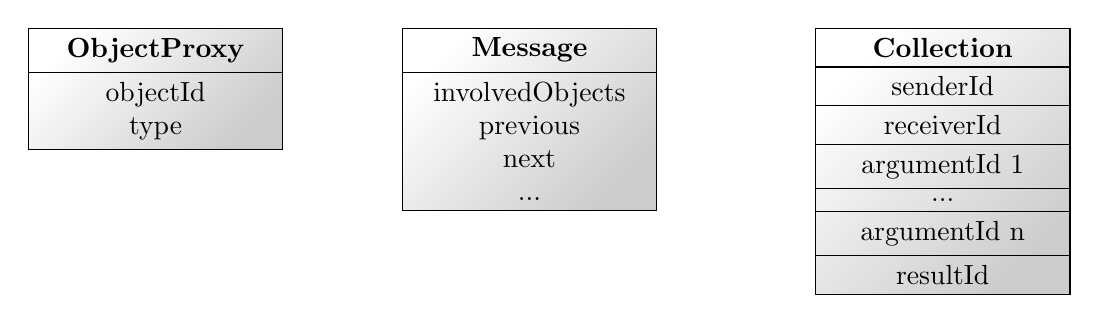
\begin{tikzpicture}[node distance=2cm]

		\node (ObjectProxy) [class, rectangle split, rectangle split parts=2] {
				\textbf{ObjectProxy}
				\nodepart{second} objectId \\ type
		};

		\node (Message) [class, rectangle split, rectangle split parts=2, below right=0cm and 1.5cm of ObjectProxy.north east] {
			\textbf{Message}
			\nodepart{second} involvedObjects \\ previous \\ next \\ ...
		};
		
		\node (Collection) [class, rectangle split, rectangle split parts=7, below right=0cm and 2cm of Message.north east] {
			\textbf{Collection}
			\nodepart{second} senderId
			\nodepart{third} receiverId
			\nodepart{fourth} argumentId 1
			\nodepart{five}...
			\nodepart{six} argumentId n
			\nodepart{seven} resultId
		};
			
	\end{tikzpicture}
	\caption[TOC Caption]{FooBar}
	\label{f:DiscussionStructure}
\end{figure}

\paragraph{Results}
\begin{figure}[h!]
	\centering
	\includegraphics[width=0.9\textwidth]{../plots/05-SpaceConsumption}
	\caption[Space Requirements Introduced Through \textsc{PathObjects}]{Additional space consumption introduced through the tracing requirements of \textsc{PathObjects} (whiskers indicate 2.5th and 97.5th percentiles).}
	\label{f:DiscussionSpace}
\end{figure}

\subsection{Threats to Validity}
The runtime measurements have been performed with the help of the \inlinecode{BlockClosure>>timeToRunWithoutGC} method.
This means that in practice, the start-up time of \textsc{PathObjects} will be slightly worse than depicted by the results of the runtime evaluation.
However, the differences are negligible, since (no long running tasks) and objects are not created and destroyed excessively.

\section{User Evaluation}
\subsection{Threats to Validity}

\section{Conditions of Use}
\label{s:Limitations}

\subsection{Metaprogramming and Reflection}
\label{ss:LimitationsMeta}
While it is not utterly impossible to trace and visualize programs that use meta-programming and reflection capabilities, the application of such techniques still might cause severe issues in conjunction with the tracing approach of \textsc{PathObjects}.


\subsection{Reliance on Test Coverage}
\label{ss:LimitationsCoverage}
Since only test cases can serve as reproducible entry points in our current prototypic implementation, only those parts of a system can be visualized that are covered by at least one test case.
In practice, this means that not all entities and execution branches that are actually in use during productive executions of the system can necessarily be visualized with existing tests.
Nonetheless, it is also feasible to write specific unit tests for the soul purpose of visualization.
Such a test then can be seen as the description of a scenario that the user wishes to examine through our tool.
However, this strategy requires that the user already has a certain degree of knowledge about the system, which might not apply when dealing with completely unknown systems. 
In such cases, one might not be able to construct a working scenario.

\subsection{Reliance on Test Quality} \todo{missing refs}
\label{ss:LimitationsTestQuality}
The best practices for unit testing and the characteristics unit tests should display enjoy broad consent throughout the agile software development community.
To name a few, they are supposed to be isolated, to be free of side-effects, to run fast, and to be reproducible, automated and unique \cite{meszaros_xunit_2006, beck_test_2002}.
However, when tests are being used as entry points for \textsc{PathObjects}, two of those recommendations become requirements.

Fast execution times are a key requirement for the applicability of our approach.
If, for instance, a test would take minutes to execute, the user would have to wait that long every time a refinement run has to be performed to collect previously unknown information.
This would possibly be still acceptable if such runs were executed only occasionally, but \textsc{PathObjects} encourages the continuous use of those features.
For example, as depicted in Section \ref{missing}, refinement runs are performed automatically as long as an object state inspector is expanded.
That means that with every step to a previously unvisited point of the execution trace, the underlying test case gets executed automatically, which in turn induces waiting time for the user in the case of long running tests. The good news is that in practice, tests usually run fast enough to make immediate feedback possible \cite{perscheid_immediacy_2010}.

The second attribute our approach presupposes is strict determinism.
Again, the main cause of concern are refinement runs.
If a test case follows divergent branches or produces objects with varying states in repeated executions, the results that are returned from such runs may be incorrect or misleading.
Admittedly, there are legitimate cases where tests are not completely deterministic, for instance when testing multithreaded applications or when working with current dates and times.
However, the \emph{record and replay} technique has been proposed to tackle this problem \cite{choi_deterministic_1998} and has successfully been adapted to the step-wise runtime analysis approach \cite{felgentreff_comparison_2012}.

\subsection{Applicability to other Programming Languages}
The fact that the prototypical implementation of our approach targets an environment that leads a niche existence raises the question to which extent the approach is transferable to other programming languages and environments.
To answer this question, one can consider the requirements \textsc{PathObjects} is based on.

First and foremost, the approach is specifically tailored to object-oriented systems.
However, a programming language does not necessarily have to feature object-oriented concepts to the same comprehensive extent that Smalltalk exhibits in order to qualify for the application of our approach.
For instance, most popular object-oriented programming languages do not expose classes as objects conceptually. 
Nevertheless, classes can readily be depicted as objects (or generally speaking: senders and receivers of messages) without impairing the expressiveness and comprehensibility of our proposed visualization.
The second requirement is the existence of reproducible entry points - which typically are available through unit tests in most development environments - and their traceability, whereas the concrete tracing technique is of no significance.

Consequently, it is fair to say that our approach is applicable to the vast majority of object-oriented programming languages.
Furthermore, since the re-implementation for other languages and platforms would undoubtedly be a tedious task, it is worth mentioning that it has been proven to be feasible to embed the existing tools of the \textsc{PathTools} framework into other development environments \cite{richter_awesome_2013}\todo{cite when available}.
The approach consists of a unified meta-model which is used to feed collected information from programs written in other target languages to the existing tools.
The only requirement is the implementation of a custom tracer and the conversion of the collected traces to the proposed meta-model.